\par\begingroup
\newcommand{\treeDiagramWidth}{0.9\textwidth}
\newcommand{\minimumNodeSize}{8mm}
\newcommand{\verticalSpacing}{10mm}
\begin{center}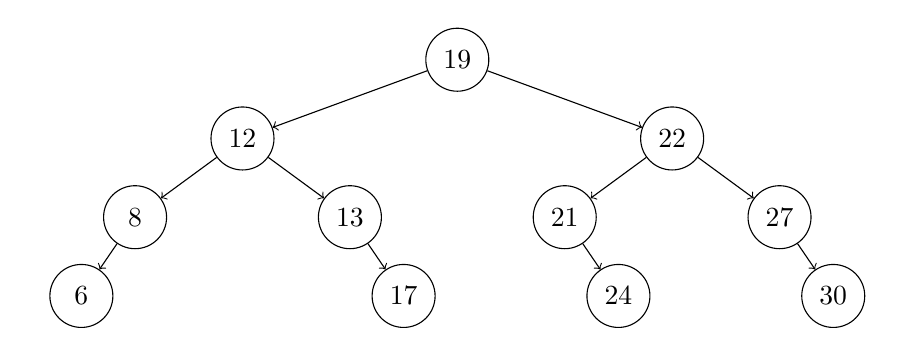
\begin{tikzpicture}
\tikzstyle{treeNode}=[minimum width=\minimumNodeSize,minimum height=\minimumNodeSize,circle,draw,inner sep=1mm]
\tikzstyle{treeEdge}=[->]
\node[minimum width=\treeDiagramWidth,rectangle] at (\treeDiagramWidth/2,0) {};\node[treeNode] (n-0-0) at ( {(\treeDiagramWidth-(\minimumNodeSize*1))/(1)*(0+0.5) + \minimumNodeSize/2 + \minimumNodeSize*0}, {-0*\verticalSpacing}) {19};
\node[treeNode] (n-1-0) at ( {(\treeDiagramWidth-(\minimumNodeSize*2))/(2)*(0+0.5) + \minimumNodeSize/2 + \minimumNodeSize*0}, {-1*\verticalSpacing}) {12};
\node[treeNode] (n-2-0) at ( {(\treeDiagramWidth-(\minimumNodeSize*4))/(4)*(0+0.5) + \minimumNodeSize/2 + \minimumNodeSize*0}, {-2*\verticalSpacing}) {8};
\node[treeNode] (n-3-0) at ( {(\treeDiagramWidth-(\minimumNodeSize*8))/(8)*(0+0.5) + \minimumNodeSize/2 + \minimumNodeSize*0}, {-3*\verticalSpacing}) {6};
\draw[treeEdge] (n-2-0) -- (n-3-0);
\draw[treeEdge] (n-1-0) -- (n-2-0);
\node[treeNode] (n-2-1) at ( {(\treeDiagramWidth-(\minimumNodeSize*4))/(4)*(1+0.5) + \minimumNodeSize/2 + \minimumNodeSize*1}, {-2*\verticalSpacing}) {13};
\node[treeNode] (n-3-3) at ( {(\treeDiagramWidth-(\minimumNodeSize*8))/(8)*(3+0.5) + \minimumNodeSize/2 + \minimumNodeSize*3}, {-3*\verticalSpacing}) {17};
\draw[treeEdge] (n-2-1) -- (n-3-3);
\draw[treeEdge] (n-1-0) -- (n-2-1);
\draw[treeEdge] (n-0-0) -- (n-1-0);
\node[treeNode] (n-1-1) at ( {(\treeDiagramWidth-(\minimumNodeSize*2))/(2)*(1+0.5) + \minimumNodeSize/2 + \minimumNodeSize*1}, {-1*\verticalSpacing}) {22};
\node[treeNode] (n-2-2) at ( {(\treeDiagramWidth-(\minimumNodeSize*4))/(4)*(2+0.5) + \minimumNodeSize/2 + \minimumNodeSize*2}, {-2*\verticalSpacing}) {21};
\node[treeNode] (n-3-5) at ( {(\treeDiagramWidth-(\minimumNodeSize*8))/(8)*(5+0.5) + \minimumNodeSize/2 + \minimumNodeSize*5}, {-3*\verticalSpacing}) {24};
\draw[treeEdge] (n-2-2) -- (n-3-5);
\draw[treeEdge] (n-1-1) -- (n-2-2);
\node[treeNode] (n-2-3) at ( {(\treeDiagramWidth-(\minimumNodeSize*4))/(4)*(3+0.5) + \minimumNodeSize/2 + \minimumNodeSize*3}, {-2*\verticalSpacing}) {27};
\node[treeNode] (n-3-7) at ( {(\treeDiagramWidth-(\minimumNodeSize*8))/(8)*(7+0.5) + \minimumNodeSize/2 + \minimumNodeSize*7}, {-3*\verticalSpacing}) {30};
\draw[treeEdge] (n-2-3) -- (n-3-7);
\draw[treeEdge] (n-1-1) -- (n-2-3);
\draw[treeEdge] (n-0-0) -- (n-1-1);
\end{tikzpicture}\end{center}
\endgroup\par
